% !TEX root = ./thesis.tex
% gaussian processes for regressions
% @author Tobias Wulf

\section{Gauß-Prozesse für Regressionsverfahren}\label{sec:gauss-prozesse-regressionsverfahren}


Das in der Arbeit zur Anwendung kommende Regressionsverfahren für Gauß'sche Prozesse, orientiert sich maßgebend, an der 2006 von Rasmussen und Williams veröffentlichter Leitliteratur \cite{Rasmussen2006}.
Vorarbeiten der \gls{gl:ags} \cite{Schuethe2020b}\cite{Schuethe2020} basieren dabei auf Winkelvorhersagen, die über den Mittelwert freien Ansatz gewonnen werden \cite{Rasmussen2006}.
Als funktionaler Entwurf des Regressionsmodells \cite{Schuethe2020}, decken die Vorarbeiten Modellinitialisierung \autoref{sec:gprinit} und Vorhersage mit Winkelkonfidenzintervall \autoref{sec:gprpred} ab. Dabei bezieht sich die Modellinitialisierung auf die Kernel-Implementierung, mittels Kovarianzfunktion nach \autoref{eq:kfun} und für die Abstandsfunktion $d_F^2$ nach \autoref{eq:df2}. Das aufgestellte Regressionsmodell ist in der Lage Simulationsergebnisse aus \autoref{ch:sensor-array-sim-imp} zu verarbeiten \cite{Schuethe2020b}\cite{Schuethe2020}. 


\vspace{2mm}
\begin{figure}[bph]
	\centering
	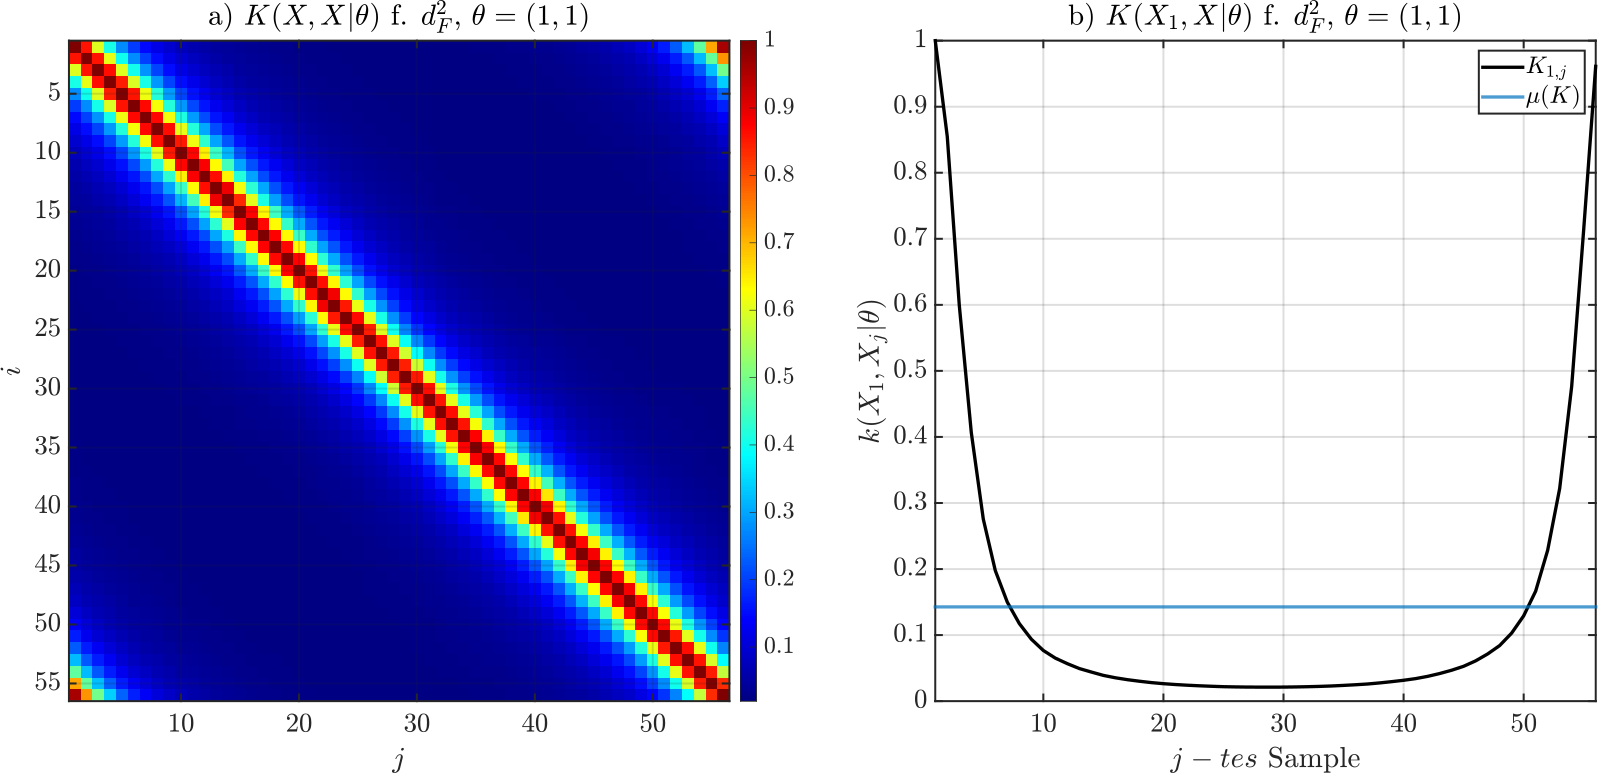
\includegraphics[width=\linewidth]{chapters/images/2-Grundlagen/Kernel-Vorabeiten-N56}
	\caption[Kernel-Implementierung der Vorarbeiten]{Kernel-Implementierung der Vorarbeiten, mittels Kovarianzfunktion $k(X_i,X_j)$ nach \autoref{eq:kfun} f. $d_F^2$ nach \autoref{eq:df2} und einen Trainingsdatensatz $X$ mit $N_{Ref} = 56$ gleich verteilten Simulationswinkeln $X_i \mapsto \alpha_i$. Die Skalierung durch Kernel-Parameter ist mit $\theta = (1,1)$ ausgeschaltet. In a) ist \autoref{alg:kmatrix} f. $K(X,X|\theta)$ genutzt und alle Trainingsdaten $X$ somit gegenseitig referenziert. Abbildung b) zeigt, Kovarianzen $K_{1,j}$ des Teildatensatz $X_1$, gegenüber sich selbst und jeden weiteren Satz $X_j$. Der Matrix-Mittelwert $\mu(K)$ in b), ist als Indikator über die gegenseitige Beeinflussung Datensätze im Regressionsverfahren zu interpretieren. Der genutzte Trainingsdatensatz $X$ basiert auf, gemachter TMR-Sensor \cite{TDK2016} Charakterisierung in \autoref{ch:tdk-datensatz}. Grafik nachempfunden aus \cite{Lang2014}}
	\label{fig:kernel-vorabeiten-n56}
\end{figure}


\clearpage


Ab hier folgt ein Wechsel der Notation um Bezüge zur Fachliteratur \cite{Rasmussen2006} zeigen zu können. Die veränderte Schreibweise ist im \autoref{sec:gprinit} unter Trainings- bzw. Testdatensätze zusammengefasst und beschrieben.
\newline
Die Parametrierung des Regressionsverfahren ist bisher empirisch ermittelt worden und stellt einen Angelpunkt in dieser Arbeit dar. Für eine selbstständige Optimierung, von Modellparametern und verbundener Modellgeneralisierung, müssen entsprechende Kriterien gebildet werden. Diese sind, in genutzter Literatur, als Minimierungsprobleme beschrieben \cite{Rasmussen2006}\cite{Guerrero2014}\cite{Lang2014}. 
\newline
Im Gegensatz zur Leitliteratur \cite{Rasmussen2006}, die Lösungsansätze für Regressionen eindimensionaler Funktionen beschreibt, ist für die Winkelvorhersage eine kombinierte Regression einer zweidimensionalen Funktion herzustellen. Da Ableitungen von Winkelstellungen, über orthogonal zueinander stehenden, Cosinus- und Sinus-Funktionen erfolgen. Dabei ist die Adaption der Array-Daten-Formate aus \autoref{sec:prinzip-des-sensor-arrays}, bereits in den Vorarbeiten gelöst worden \cite{Schuethe2020} und über die Kovarianzfunktion \autoref{eq:kfun} für $d_F^2$ \autoref{eq:df2} implementiert. \autoref{fig:kernel-vorabeiten-n56} zeigt die Implementierung aus den Vorarbeiten, anhand der Kovarianzfunktion und resultierender Kovarianzmatrix, für ein Beispiel eines $N_{Ref} = 56$ Observierungen großen Trainingsdatensatz. Für diese Implementierungsform, wäre das ein viel zu großer Datensatz in der realen Anwendung. In Bezug auf das Sensor-Array \autoref{sec:prinzip-des-sensor-arrays}, müssten $2 \times 56 = 112$ Matrizen abgelegt werden, sodass diese dem Regressionsprozess als Referenzen zur Verfügung stehen. Was hier zwar ein drastisches Beispiel ist, dass allerdings sehr schön das Verhalten der Kovarianz in Verbindung mit TMR basierten Daten zeigt.
\newline
Die Kovarianzfunktion mit resultierender Kovarianzmatrix, muss in der Lage sein systemische Eigenschaften wiedergeben zu können. Auf den TMR-Sensor \cite{TDK2016} gemünzt, muss die Matrix einfach periodisch sein. Das ist durch Kurvenverlauf in \autoref{fig:kernel-vorabeiten-n56} b) und durch ansteigenden Ecken links unten und rechts oben in a) zu erkennen. Es gibt nur eine vollwertige Diagonale. Bei Systemen höherer Periodizität, müsste die Kovarianzfunktion, entsprechend mehrere dieser Diagonalen, durch Superposition oder Trigonometrie-Funktionen erzeugen \cite{Rasmussen2006}.


\clearpage


Die homogenen Bereiche der Matrix zeigen, dass die Trainingsdaten $X$ mit gleichbleibender magnetischer Stimulanz erzeugt wurden. Gäbe es Fehllagen in der Erzeugung, Sprunghaften Versatz des Sensor-Arrays, oder Verkippung des Magneten, wären die Flächen unterbrochen. Ebenfalls indiziert die durchgehende Diagonale, dass die Rotation konstant mit gleichbleibenden Abständen vollzogen worden ist. Würden Sprünge in der Rotation auftauchen, müssten diese durch Schnitte in der Diagonale und eventuell durch Absenkungen der Ecken ersichtlich werden. Durch Bruch in der Periodizität würden Ecken der Matrix ganz verschwinden.


Der annähernd keilförmige Kurvenverlauf in \autoref{fig:kernel-vorabeiten-n56} b), bei ausgeschalteter Skalierung $\theta = (1,1)$, weißt auf ein System mit einfacher Komplexität hin \cite{Rasmussen2006}. Das heißt, es benötigt entweder eine erhöhte Anzahl von Trainingssamples, oder eine Parameteroptimierung und aufbohren der Modellkomplexität, um von den Trainingsdaten abweichende Daten, mit geringen Regressionsvarianzen prozessieren zu können \cite{Rasmussen2006}. Andersherum gesagt, gibt man alle möglichen in Winkelpositionen über die Trainingsdaten vor, muss der Regressionsfehler automatisch gegen null gehen. Die Modellanpassung auf eingespeiste Trainingsdaten, sowie gleichzeitige und sinnvolle Verringerung des Datenumfangs, bilden dabei die zu haltende Balance in Bezug auf akzeptable Winkelfehler \cite{Rasmussen2006}. 

 